\documentclass[10pt]{extarticle}
\usepackage{amsmath}
\usepackage{extsizes}
\usepackage{graphicx}
\usepackage{textcomp}
\usepackage{tikz}
\usepackage[margin=0.4in]{geometry}

\usepackage{nopageno}
\usepackage{multicol}

\title{MATH235 Course Summary}
\date{}
\author{Public ID: 93}
\begin{document}
\pagenumbering{gobble}
\maketitle
\newpage
\pagenumbering{arabic}

\begin{multicols}{2}
\section{Differential Equation Intro}
\subsection{Wait, what are they?}

A differential equation establishes a relationship between value and the way it
changes. A function models value from another independently-changing value, and
the derivative of the function describes the rate of change of the dependent
value with respect to the independent value. 

Imagine what would happen if a function were set equal to its own derivative.
This process marks the birth of a differential equation---before solving it,
be sure to send your congratulations on the parents' new arrival. Now, {\em
what sort of function spits out the same value and slope for any value you plug
in?}

\begin{equation*}
    y(t) = e^t
\end{equation*}

0 also does the trick, but it isn't as exciting. This also denotes a particular
solution to this problem of y' = y.


\subsection{Wait, particular solution?}

Yeah. Notice how when you differentiate something like \(2e^t\), you still get
\(2e^t\)? Turns out, you can slap on any real coefficient and the solution
won't budge. This means our solution of \(e^t\) only gives us a finite picture
of infinite solutions. To remedy this, we can add an {\em arbitrary constant}.
It's good practice to call it C, but you can get away with using any
Latin-derived character, or even Greek or Cyrillic if you desire spicing up
your nomenclature.

\begin{equation*}
    y(t) = Ce^t
\end{equation*}

Everything's good now, having found the {\em general solution}. But,
unfortunately, this does not exhaust the entire differential equation doctrine.
Be sure not to miss my next sermon for a fuller picture.


\subsection{But this is written text, everything is already in the document}

Same deal with textbooks, why don't you read one of those instead?


\subsection{...Okay, fine, I've left and now I'm back}

Welcome. To be able to broaden our scope of ordinary differential equation
solving beyond intuition, we need to define a few kinds of differential
equations first.


\section{Differential Equation Classification}

\subsection{Order}

The rank of "order" of a differential equation is simply the count of
successions of differentiating the dependent variable. y', or for the Leibniz
proponents, \(dy/dx\), is the first derivative of y. If this is the highest
succession of derivatives found in the differential equation, then it is {\em
first order}. This document will really only cover first order and second order
differential equations.


\subsection{Autonomy}

The name is indicative of the behavior. When you have an autonomous
differential equation, the dependent variable is self-governing, indifferent to
any state of the independent variable. However, when it comes time to solve the
differential equation, this independent variable is sometimes necessary to
properly model its behavior as a function, like with the first example. 


\subsection{Linearity}

This can be most easily defined by the form of a first order linear
differential equation. It must be in or can derive to this form:

\begin{equation*}
    \mathbf{F}(\vec{y}, t) = \mathbf{A}(t)\vec{y} + \vec{b}(t)
\end{equation*}

There's a lot of emboldening and h{\em arrow}ing symbols that you may not be
familiar with. Don't worry, this is just the most general form which can assume
a much-friendlier appearance with the assumption of variable dependence and
single-dimensionality. Here's a nicer-looking, more specific case of first
order linearity:

\begin{equation*}
   y' = f(t)y + g(t) 
\end{equation*}

Very friendly, but very specific. That tends to be a recurring trend in
differential equations; it's just something you have to get used to.


\subsection{Homogeneity}

We can piggyback off of the definition of linearity to define homogeneous
differential equations. For first order cases:

\begin{equation*}
    \mathbf{F}(\vec{y}, t) = \mathbf{A}(t)\vec{y}
\end{equation*}

Notice how the equation is the same, except for the lack of \(\vec{b}(t)\). For
the more specific case:

\begin{equation*}
   y' = f(t)y 
\end{equation*}

The \(g(t)\) is missing here instead. It's that simple! Now you're ready to
solve differential equations.


\subsection{Cool, but wait, how can I use this to solve differential
equations\textinterrobang}

Sorry, I got ahead of myself there. I need to show you the various {\em
methods} of solving these things. The giants have plenty of room on their
shoulder, hop on!


\section{Differential Equation Methods}

\subsection{Separation of Variables}

This is a natural starting place to the venture to solving differential
equations on your own! While it only pertains for us to a certain flavor of
differential equations (first order, separable, and ordinary),
it is a rather intuitive method with some background of Calculus. Our first
example can serve nicely as yet another example, but with a twist!

\begin{equation*}
    \dfrac{dy}{dt} = yt
\end{equation*}

This differential equation is linear, homogeneous, but most importantly, {\em
separable}. Yesiree, this basically means that all of the y terms can stay on
one side of the equation, and all of the t terms can stay on the other side.
Separated but equal. Here's what the end result looks like:

\begin{equation*}
    \dfrac{dy}{y} = tdt
\end{equation*}

If only we knew how to indefinitely add up an arbitrarily small change in a
variable... oh yeah, Calculus!

\begin{equation*}
    \int\dfrac{dy}{y} = \int tdt
\end{equation*}

This ends us up with:

\begin{equation*}
    ln|y| = t^2 + C
\end{equation*}

Yes, a constant is necessary when antidifferentiating, but two aren't necessary
because this can just simplify to yet another constant. Hence, the C stays
where it is most convenient, where the t terms lie.

\begin{equation*}
    y(t) = e^{t^2 + C} = C_1e^{t^2}
\end{equation*}

And this is the end result for the general solution for the differential
equation. Exponent rules can place another C as a coefficient to the exponent,
and exponentiating both sides can give us an explicit solution.


\subsection{Method of Integrating Factors}

Like my grandmother always used to say: "You're out of luck on integrating
factors if you can't get a differential equation into an explicitly linear
form." And how. We can use the specific definition of a linear differential
equation as a starting point for this method:

\begin{equation*}
    y' = f(t)y + g(t) 
\end{equation*}

Now close your eyes, I'm going to change it a bit, but it will still stay
ultimately the same. Promise me you're gonna do it.

Okay, you can open them now. Notice anything different?

\begin{equation*}
    y' + f(t)y = g(t) 
\end{equation*}

That's right. There has been a shift in the expression,
but it's still the same ol' generic linear differential equation we
know and love. Without getting into the proof of why this method actually
works, I'm going to throw in the result of the proof that makes differential
equations in this form trivial to solve in certain linear cases:

\begin{equation*}
    \mu = e^{\int{}f(t)dt}
\end{equation*}

And that is what I mean. Sure, if you have a constant or inverse y in that
f(t), it'll be smooth sailing, but things might get hairy with trig or
high-order polynomials, as you'll be needing to antidifferentiate the result
again afterwards!

After having solved that, all that is left to do is derive y from this
equation:

\begin{equation*}
    \mu y = \int \mu g(t) dt
\end{equation*}

Simple enough. The worst you may have to do is integration by parts---and
otherwise---it either isn't possible with your typical antidifferentiation
methods or not worth the hassle.

\subsection{Method of Undetermined Coefficients}

Like any superhero, this method does not stand alone. In fact, it is more
analogous to a sidekick---cleaning up the mess after a job well done. This {\em
mess} is none more than a nonhomogeneous component of a differential equation.
Oftentimes, this takes longer to figure out than the homogeneous part! Our
silent, studious knight has kept in the shadows for long enough; in this
section, our underdog will get the spotlight that it finally deserves. How does
it get the task done? Guessing.

\begin{equation*}
    y' - y = e^{2t}
\end{equation*}

Hey look, a nonhomogeneous differential equation! How convenient for it to drop
by in a trying time like this. To solve this using the Method of Undetermined
Coefficients, we have to first {\em not} use it. Let's get rid of the
nonhomogeneous part, \(e^{2t}\). Just change it to 0. Make it disappear. Now it
is homogeneous. Now solve!
    
\begin{equation*}
    y_h(t) = Ce^t
\end{equation*}

That's a job for another method, though. After having found the {\em
homogeneous} solution, we now need to use this method for the stuff we set to
0, \(e^{2t}\). Remember the particular solution vs. general solution stuff I
talked about a while ago? This is a good time to apply it in the real world of
mathematics. We need to make the \(e^{2t}\) general to find a certain
particular solution! That means an arbitrary constant must be tacked onto it.
Let's make it \(A\).

\begin{equation*}
    y_p(t) = Ae^{2t}
\end{equation*}

This is our best attempt right now at a "particular" solution. To find out if
it works, we need to see if it's possible to find the values of the arbitrary
constants so that it {\em is} particular. We take our guess and treat it as the
y in the differential equation, and set it equal to the nonhomogeneous piece. 

\begin{equation*}
    2Ae^{2t} - Ae^{2t} = e^{2t}
\end{equation*}

With some algebra, we can deduce that \(A\) is equal to 1. The solution to this
problem is defined by this method as the sum of the particular and general
solutions found:

\begin{equation*}
    y(t) = Ce^t + e^{2t}
\end{equation*}

And Gotham is yet again saved from prompt and utter destruction. Not
necessarily because of the Method of Undetermined Coefficients, but are you
prepared to assume responsibility for the loss of millions of lives if that
actually turned out to be the case?


\subsection{Characteristic Equation}

This method is exclusively for second order linear differential equations. Keep
away if you have anything else! You're gonna need to have it in this form:

\begin{equation*}
    Ay'' + By' + Cy = f(t)
\end{equation*}

And a-one, and a-two, and alakazam!

\begin{equation*}
    Ar^2 + Br + C = 0
\end{equation*}

You're now looking at your friendly neighborhood characteristic equation.
Finding the value(s) of r will set you well on your way to finding the
homogeneous solution, where the Method of Undetermined Coefficients can take
care of the rest if need be. But what do you {\em do} with the r's once you
have them? It depends on their value, of course. The following expressions will
{\em express} which solution form you'll need:

\begin{equation*}
    \text{Real: } C_1e^{r_1t} + C_2e^{r_2t}
\end{equation*}
\begin{equation*}
    \text{Repeated: } C_1e^{rt} + C_2te^{rt}
\end{equation*}
\begin{equation*}
    \text{Complex: } C_1e^{\alpha t}\text{cos}(\beta t) + 
    C_2e^{\alpha t}\text{sin}(\beta t)
\end{equation*}

In the complex case, the $\alpha$ and $\beta$ refer to the real and imaginary
components of the conjugate root pair, respectively. Don't worry that there are
two roots, either---it's only a sign change in the imaginary, which is
equivalent to a sign change in the expression's coefficient. The C, being
arbitrary, is indifferent to this. Don't fret, big C can handle it!


\subsection{Laplace Transforms}

When all else fails, or if you really enjoy solving for partial fractions,
Laplace can get the job done. There are two components to using Laplace
Transforms: finding the transforms and using them to solve for differential
equations. Let's focus on the latter, as people will usually have a transform
table at hand to get your differential equation in Laplace land. Just ask!

Laplace transformation basically changes a function of time into a function of
frequency. This is an important tool for finding solutions to a differential
equation with piecewise behavior, as typical methods do not play nicely with
this. Play us off, Dirac!

\begin{equation*}
    y' = \delta_{1}, y(0) = 2
\end{equation*}

And he does so with an instantaneous value of 1 at \(t = 1\), and 0 everywhere
else. In our Laplace land of frequency, this is equivalent to \(e^{-s}\).
Very quaint, but what can we do with this to solve the differential equation?
By putting everything else into Laplace land:

\begin{equation*}
    sY(s) - y(0) = sY(s) - 2 = e^{-s}
\end{equation*}

Solving for \(Y(s)\) will get us to a point where taking us out of Laplace land
will turn \(Y(s)\) into \(y(t)\). With the other side possible to transform
back as well, the differential equation is solved!

\begin{equation*}
    Y(s) = \dfrac{e^{-s}}{s} + \dfrac{2}{s} \rightarrow  y(t) = u_1(t) + 2
\end{equation*}

What is that strange \(u_1(t)\) function? It's a step function, my dear Watson.
Instead of a different {\em value} for only an infinitesimal time, there's
instead an infinitesimal {\em change in value}, at \(t = 1\) again as noted in
the subscript. Before the t, the value is 0, and after the t, it is 1. Solving
differential equations with these two type of functions will almost always give
you solutions with them still in it. After all, how else will it describe the
behavior? 


\subsection{Eigenvalues and Eigenvectors}

If you thought modeling behavior with successive derivatives wasn't enough to
wrap your head around, let's now try it with more than one dimension! A matrix
will let us do this, which is just a table which lets us do some cool math if
we abstract it to a list of equation coefficients.  This is also where our
general definition of single order linearity can help us out.

\begin{equation*}
    \mathbf{F}(\vec{y}, t) = \mathbf{A}(t)\vec{y} + \vec{b}(t)
\end{equation*}

But again, let's cut out some of the fluff that does not concern us in very
simple cases:

\begin{equation*}
    \dfrac{d \mathbf{Y}}{dt} = \mathbf{A}y
\end{equation*}

To keep our discussion within the scope of differential equations, instead of
linear algebra, I'll just state how to find the values that are necessary to
solve for one of these, in flow chart form! It can be found in the back of the
document.


\subsection{In summary}

How about a Venn diagram, showing what methods you should use under a variety
of differential equations? All expenses are paid; take it! You can also find it
in the back of the document.

Each method under its collection of categories aren't necessarily guaranteed to
work, like separation of variables if nonseparable, but it gives a pretty good
idea of the methods to try. Matrix stuff is also not included as it's easier to
treat it as mutually exclusive to single-dimensional differential equations.


\section{Conclusion}

It now seems like you're ready to tackle on the world's problems. Equip your
Ticonderoga and set sail!


\subsection{It's all in a day's work}

It's a far cry from easing geopolitical tensions, but all research
finds its application somewhere. Differential equations  can give us models,
which behave not entirely unlike our chaotic existence. There are an
arbitrarily large amount of variables that can go into "modeling" our real
world. Can we pinpoint them all? Maybe, but it would be awfully inconvenient to
have to simulate the entire observable universe in order to retrieve the exact
behavior of a mass-spring system. Or maybe it eventually won't; that would be
exciting!


\subsection{But I digress}

Differential equations are an invaluable tool for modeling behavior based on
initial conditions, the behavior of an independent variable, and its own
behavior. Where would MATH235 be without it?

\end{multicols}


\begin{tikzpicture}
    \begin{scope}[blend group=soft light]

    \fill[black!25!white] ( 90:2.5) circle (4); 
    \fill[black!25!white] (210:2.5) circle (4);
    \fill[black!25!white] (330:2.5) circle (4);

    \end{scope}

    \node at ( 90:7) {\textbf{First order}}; 
    \node at (210:7.7) {\textbf{Homogeneous}}; 
    \node at (330:7.2) {\textbf{Linear}};

    \node at (35:2.8) {Integrating factors};
    \node at (270:2.2) {Integrating factors};
    \node at (270:2.6) {Separation of var.};
    \node at (208:4.7) {Characteristic equation};

    \node {Separation of var.};
    \node at (330:4.5) {Undetermined coefficients};
    \node at (145:2.5) {Eyeballing it};

    \node at (145:7.5) {Laplace Transforms}; 
    \node at (148:7.5) {(and everywhere else)}; 
    \node at(90:4.5) {Separation of var.};

\end{tikzpicture}

\small{Generated with tikzpicture package}


\hfill

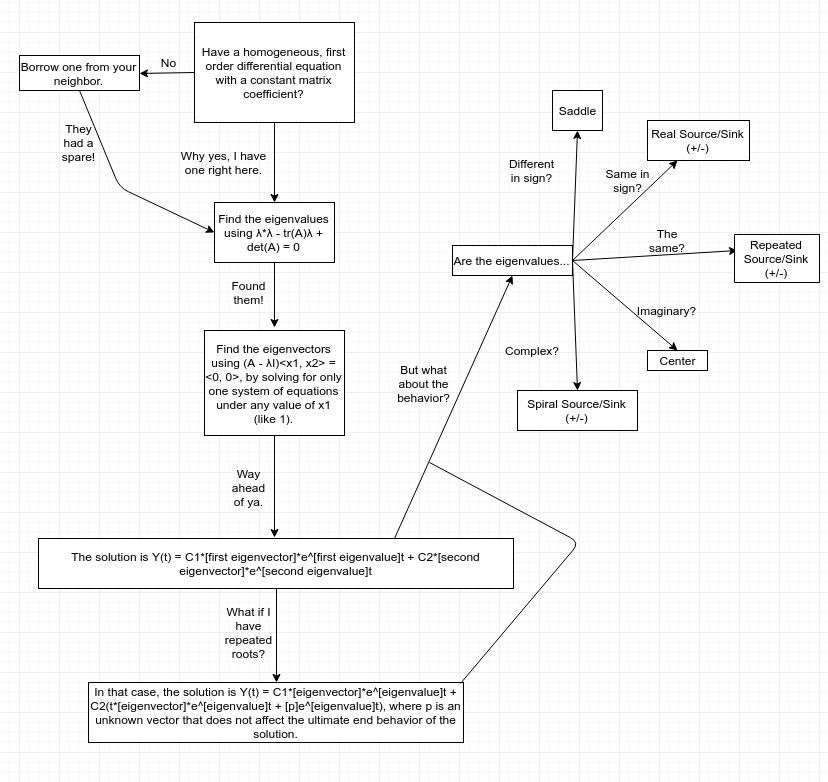
\includegraphics[width=\textwidth,height=\textheight,keepaspectratio]{flow}

\small{Generated with draw.io}

\hfill


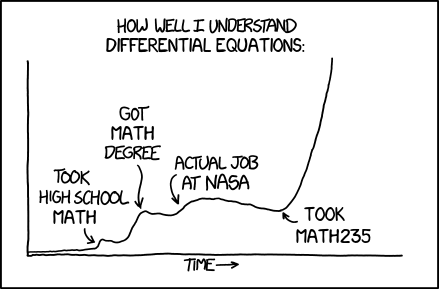
\includegraphics{xkcd}

\small{Courtesy of https://xkcd.com/1356/}


\end{document}
